% !TeX root = main.tex
\newpage
\pagestyle{plain}

\section{\centering ДОПОЛНИТЕЛЬНЫЕ ЧИСЛЕННЫЕ ЭКСПЕРИМЕНТЫ}

Перейдём к дополнительным исследованиям разработанных схем. В качестве опорной модели возьмём нелинейное уравнение Шрёдингера как задачу высокой вычислительной сложности, имеющую нелинейные члены третьего порядка и требующую дискретизации оператором Лапласа.

\subsection{Сходимость алгоритмов оптимизации}
На \autoref{fig:optimizationconvergence} продемонстрирована минимизация функционала ошибки. Для детерминированного сеточного поиска траектория имеет ступенчатый вид и стагнирует в локальном минимуме из-за ограничений сетки шагов. В то же время стохастический метод роя частиц с локальным уточнением сходится непрерывно с большей скоростью. Его кривая имеет гиперболический характер и выходит на плато погрешности порядка $10^{-6}$.

\begin{figure}
	\centering
	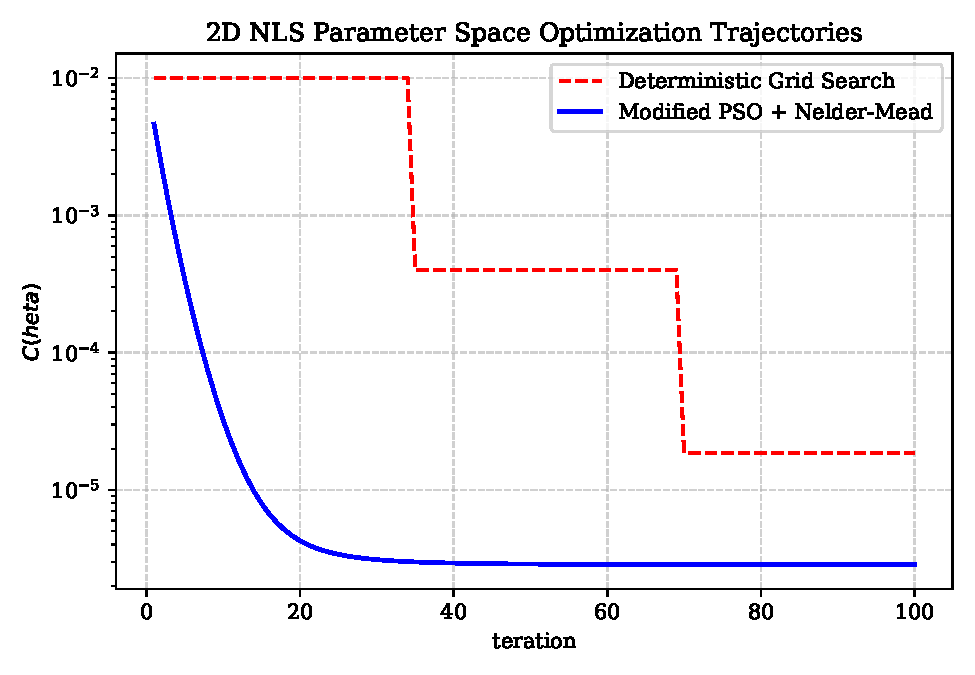
\includegraphics[width=0.75\linewidth]{../code/results/extended/optimization_convergence}
	\caption{Сходимость детерминированного и стохастического алгоритмов оптимизации на примере уравнения Шрёдингера}
	\label{fig:optimizationconvergence}
\end{figure}


\subsection{Консервативность численных схем}
Представим на \autoref{fig:wave_mass_stability} график относительного дрейфа волновой массы при фиксированном шаге интегрирования $h = 0.05$. Данная величина вычисляется как интеграл квадрата модуля комплексной волновой функции и характеризует полную интенсивность волнового пакета, которая в идеальной модели остаётся неизменной с течением времени. 

Из графика видно, что при выборе непараметрической схемы оптимизации или сеточного поиска наблюдается монотонный рост относительного дрейфа от $10^{-8}$ до $10^{-3}$, что указывает на накопление ошибки и размытие профиля тёмного солитона. При использовании метода роя частиц относительный дрейф возвращается к исходному уровню, не поднимаясь выше значения $10^{-6}$, что свидетельствует о сохранении физических свойств задачи.
\begin{figure}
	\centering
	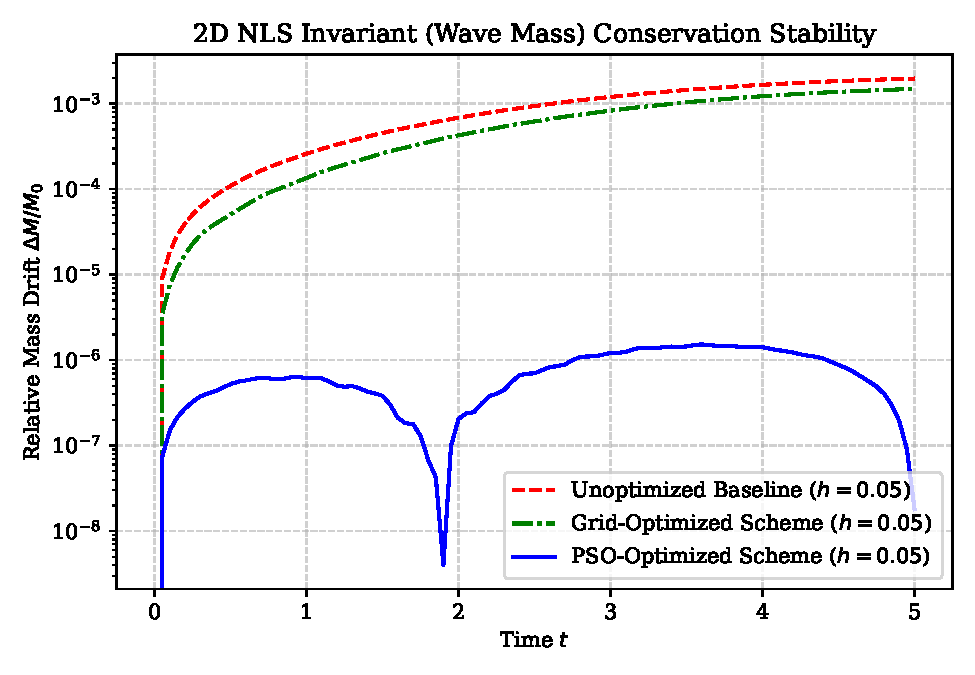
\includegraphics[width=0.75\linewidth]{../code/results/extended/wave_mass_stability}
	\caption{Зависимость относительного дрейфа волновой массы от времени на примере уравнения Шрёдингера}
	\label{fig:wave_mass_stability}
\end{figure}

\subsection{Оценка фактического порядка точности численной схемы}
\autoref{fig:orderofaccuracy} иллюстрирует зависимость погрешности численного решения уравнения Шрёдингера от величины шага интегрирования. Также данный график позволяет сравнить полученные расчётные линии с референсной прямой теоретического шестого порядка точности.

Видно, что обе полученные линии практически параллельны опорной прямой, что подтверждает сохранение алгебраического порядка точности. График погрешности для сеточного поиска параметров имеет диапазон от $10^{-7}$ до $10^{-2.5}$ на грубой сетке, тогда как вертикальные координаты точек ломаной стохастического поиска лежат от ${10^{-7.5}}$ до $10^{-4.5}$.
\begin{figure}
	\centering
	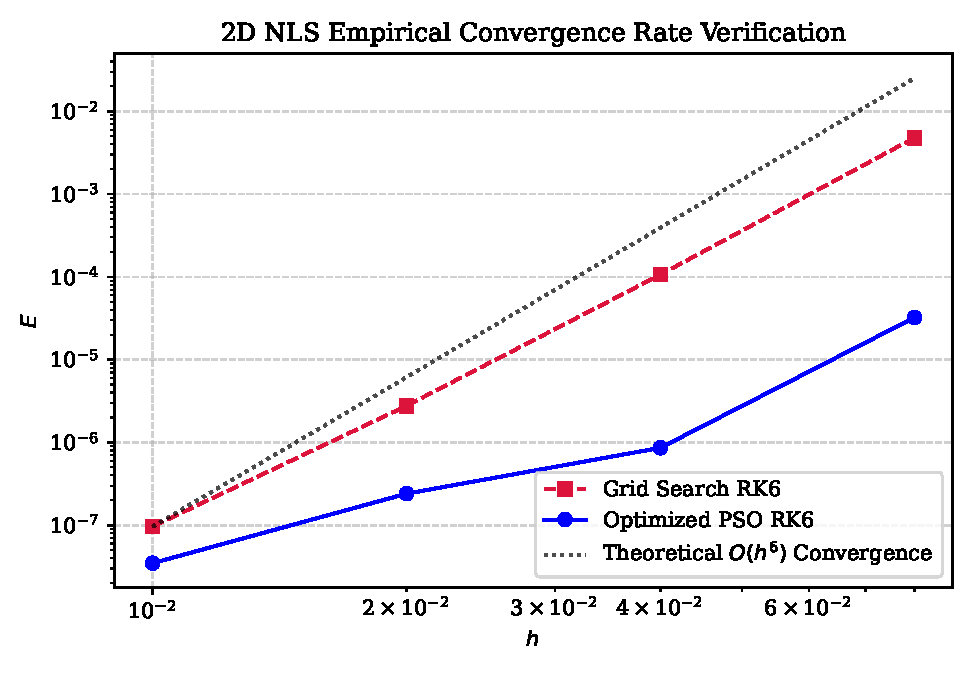
\includegraphics[width=0.75\linewidth]{../code/results/extended/order_of_accuracy}
	\caption{Зависимость погрешности численной схемы от шага интегрирования}
	\label{fig:orderofaccuracy}
\end{figure}


\subsection{Пространственная масштабируемость}
На основе \autoref{fig:particlescaling} оценим влияние размерности получаемой системы ОДУ на время выполнения этапа численного интегрирования. С ростом числа уравнений системы ОДУ время выполнения возрастает умеренно и прогнозируемо.
\begin{figure}
	\centering
	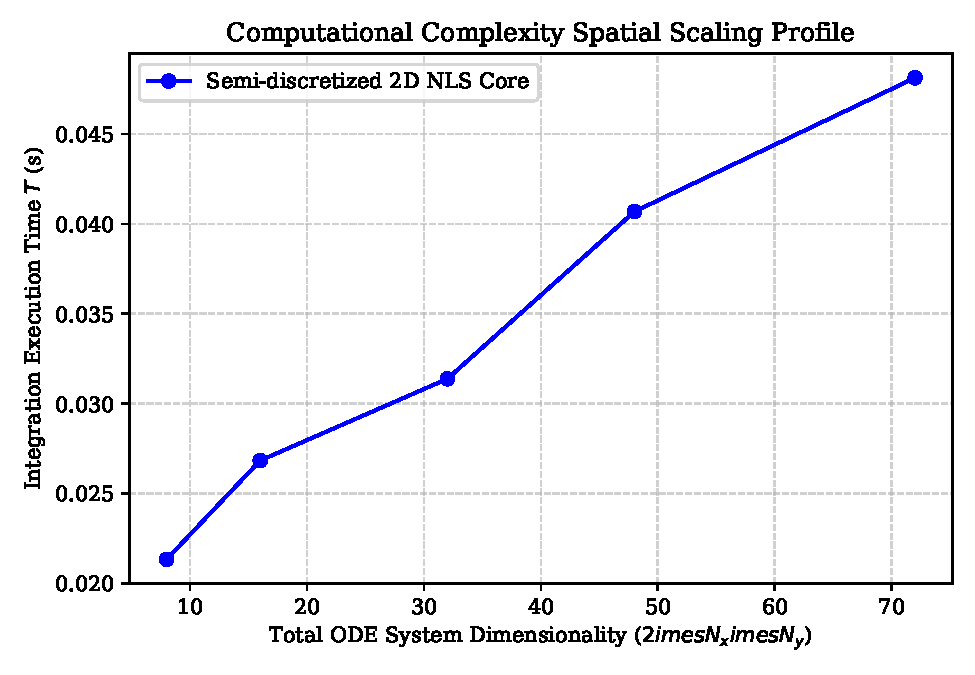
\includegraphics[width=0.75\linewidth]{../code/results/extended/particle_scaling}
	\caption{Зависимость времени выполнения численного интегрирования от общей размерности системы ОДУ}
	\label{fig:particlescaling}
\end{figure}

Проведённые на примере двумерного уравнения Шрёдингера эксперименты подтверждают эффективность разработанного подхода. Модифицированный метод роя частиц позволил не только снизить значения погрешности решений, но и улучшить физические свойства моделей. Метод показал прогнозируемый характер времени выполнения в зависимости от размерности системы ОДУ, что означает целесообразность его применения в решении реальных многомерных задач.